% Template for ICIP-2014 paper; to be used with:
%          spconf.sty  - ICASSP/ICIP LaTeX style file, and
%          IEEEbib.bst - IEEE bibliography style file.
% --------------------------------------------------------------------------
\documentclass{article}
\usepackage{spconf,amsmath,graphicx}

% Example definitions.
% --------------------
\def\x{{\mathbf x}}
\def\L{{\cal L}}

% Title.
% ------
\title{SVETLANA: a Supervised Segmentation Classifier for Napari}
%
% - STALIN
% - SALSIFI
% - SALSA
% - SCAN
% 
% ---------------
\name{Clément Cazorla, Pierre Weiss, Renaud Morin\thanks{Thanks to XYZ agency for funding.}}
\address{Imactiv-3D, IMT}
%
% Two addresses (uncomment and modify for two-address case).
% ----------------------------------------------------------
\twoauthors
 {Clément Cazorla, Renaud Morin \sthanks{C. Cazorla is partially funded by ANR CIFRE 2020/0843.}}
	{IMACTIV-3D\\
	1 place Pierre Potier, 31100 - Toulouse}
 {Pierre Weiss \sthanks{P. Weiss acknoledges a support from ANR-3IA Artificial
and Natural Intelligence Toulouse Institute and ANR Micro-Blind}}
	{CNRS \& Université de Toulouse\\
	31400 - Toulouse}

\begin{document}
%\ninept
%
\maketitle
%
\begin{abstract}
We develop and present a Napari plugin called SVETLANA (SuperVised sEgmenTation cLAssifier for NapAri). It is dedicated to the manual or automatic classification of segmentation results in bio-medical imaging.
While many open-source softwares now make it possible to automatically segment complex 2D and 3D objects such as cells in biology, the subsequent analysis of the results is not yet accessible to non specialists. 
This plugin allows end-users to train and use efficient neural network classifiers such as residual networks. 
The resulting network can be used as a post-processing tool to improve the segmentation, or as a classifier for various tasks (e.g. separating different cell populations).
We showcase its practicality through various real cell biology problems in 2D, 3D and multi-spectral imaging.
\end{abstract}
%
\begin{keywords}
Segmentation, Classification, Convolutional Neural Networks, bio-medical imaging
\end{keywords}
%
\section{Introduction}
\label{sec:intro}

The last decade has made automatic segmentation of bio-medical images much more accessible to users not familiar with signal processing. 
This is the result of progress in machine learning, to the creation of open training databases and to the development of ergonomic open-source softwares. Technologies such as neural networks provide unprecedented segmentation results. They make it possible to avoid setting hyperparameters which are often hard to tune and interpret. 
Examples of powerful and popular tools for segmentation in biology include Ilastik \cite{berg2019ilastik}, CellPose \cite{stringer2021cellpose}, StarDist \cite{fazeli2020automated} or Deep-ImageJ \cite{gomez2021deepimagej}. 

\subsection{Our motivation}

Unfortunately, segmentation masks -- as good as they are -- are rarely directly exploitable to answer biological questions. In particular, it is often necessary to classify the detected objects in order to perform statistical analyses that give a concrete meaning to the results. 
While these excellent segmentation tools have solved an important problem, a difficult part of the analysis remains inaccessible to most users.

\subsection{Our contribution}

The goal of this work is to continue filling the gap between methodological advances and end-users, by providing convenient tools for the classification of segmentation results. 
We resort to the newborn Napari environment \cite{perkel2021python} which allows visualizing and analyzing complex multi-dimensional images (e.g. 2D, 3D, 3D+t, hyperspectral) in Python.
Our software takes the form of a Napari plugin called SVETLANA. 
It is separated in three different modules: 
\begin{description}
  \item[\emph{Annotation}] This module picks connected components of the segmentation masks at random and displays them within their neighborhood, so that the user can label them. In our 2D experiments, it allows labelling about 1000 cells in 15 minutes.
  \item[\emph{Training}] This module allows to pick an arbitrary Pytorch \cite{paszke2019pytorch} neural network architecture (possibly pretrained) and to further train it with the annotations generated by the previous module.
  \item[\emph{Prediction}] This module uses the trained network to classify the connected components of the segmentation mask.
\end{description}
The results are stored in files widely accessible formats for the forth-coming analyzes. This plugin meets a need to further enhance the excellent results obtained with recent wide purpose segmentation tools.

\subsection{Related works}

Different options can be adopted to segment and classify objects in images. 
Before 2010, most of the works relied on the following pipeline (see e.g. \cite{irshad2013methods}): 1) Segment the image 2) Annotate the resulting masks 3) Extract features within the masks (e.g. edges, textures, ...) 4) Design a classifier based on the extracted features. 
Each of the above step was carried out with carefully hand-crafted methods. 
Supervised and unsupervised learning then progressively entered in the game. 
In many cases, they outperformed man-made routines by allowing to explore a wider range of decision routes. 

An effort was then pursued to make these technologies available to the larger number. One remarkable example is Ilastik \cite{berg2019ilastik}. There, a few annotations by the user are usually enough to perform complex classification tasks with an arbitrary number of classes. Its backbone is a random forest classifier with a fixed number of features (convolutions with different filter types). It is widely praised for its ease of use. A few clicks are enough to solve many real-world problems. Unfortunately, this strength is also a limitation in certain cases: the performance of random forests falls short in comparison with the most advanced segmentation and classification routines trained with vast collection of carefully labelled data. 

When precision is critical, the rapidly evolving state-of-the-art is rather based on neural networks and especially convolutional neural networks \cite{dhillon2020convolutional,8237584}. The downside of these technologies is the need to create large datasets, which are usually just not accessible. Each biology laboratory explores a different organism, at a different scale with a different modality and focus. Each collected image can be costly both in terms of money, know-how and time. To address this issue, new initiatives emerge to collect large heterogeneous training databases. For instance the Data Science Bowl \cite{caicedo2019nucleus} allowed to train a single neural network, which is now capable of segmenting cells of nearly any type. This tool, embedded in neat graphical interfaces (e.g. CellPose \cite{stringer2021cellpose} or StarDist \cite{fazeli2020automated}) is a huge asset for biology. 


\section{Plugin description}
\label{sec:format}
{}
The objective of SVETLANA as a whole is to provide a tool to "sort" the segmentation results, either manually or automatically. 
It is separated in 3 different stages, similar to what is done in Ilastik \cite{berg2019ilastik}. 
\subsection{The annotation}

This first sub-plugin takes as input two images: the image itself and its segmentation mask. Each object ot the latter should be given a different label. For instance, a 20-cell image would have a mask with values in a range of 0-20.
\\
There are two philosophies for using this software:
\begin{itemize}
  \item It can be seen as an annotation tool in its own right. For an image with a reasonable amount of segmented objects, it could be used to classify them in a simple and efficient way, in order to perform statistical analyses afterwards.
  \item Nevertheless, if the image contains an astronomical number of detected objects, this software becomes an aid for the creation of a training data set for a classifier. Indeed, the tool extracts a subset of thumbnails of a size chosen by the user and randomly selected in order to maximize the chances of obtaining a minimal and representative data set. 
\end{itemize}

As shown in \ref{labelization}, since it is not easy for the user to determine the optimal patch size, there is a feature to suggest it to the user, as well as the maximum number of thumbnails that can be extracted, i.e. the number of objects of which the segmentation mask is composed. 

It works on 2D and 3D images, whatever the channels number. Each patch represents the object in its neighbourhood, as shown in \ref{patch}. Tne user can choose the maximum label number he wants, and each label is attributed licking on the number we want to give him. Each time a label is goven, the next image is automatically loaded. If an error is commited, a backward step is possible by clicking on the "r" key.

Once the patches have been extracted and the annotation completed, it is possible to save a new mask per existing label, as well as a binary file that can be reloaded using the torch.load() function. It contains morphological features of interest of each of the objects that were extracted from the connected component analysis.

\begin{figure}[htp!]
 \centering
 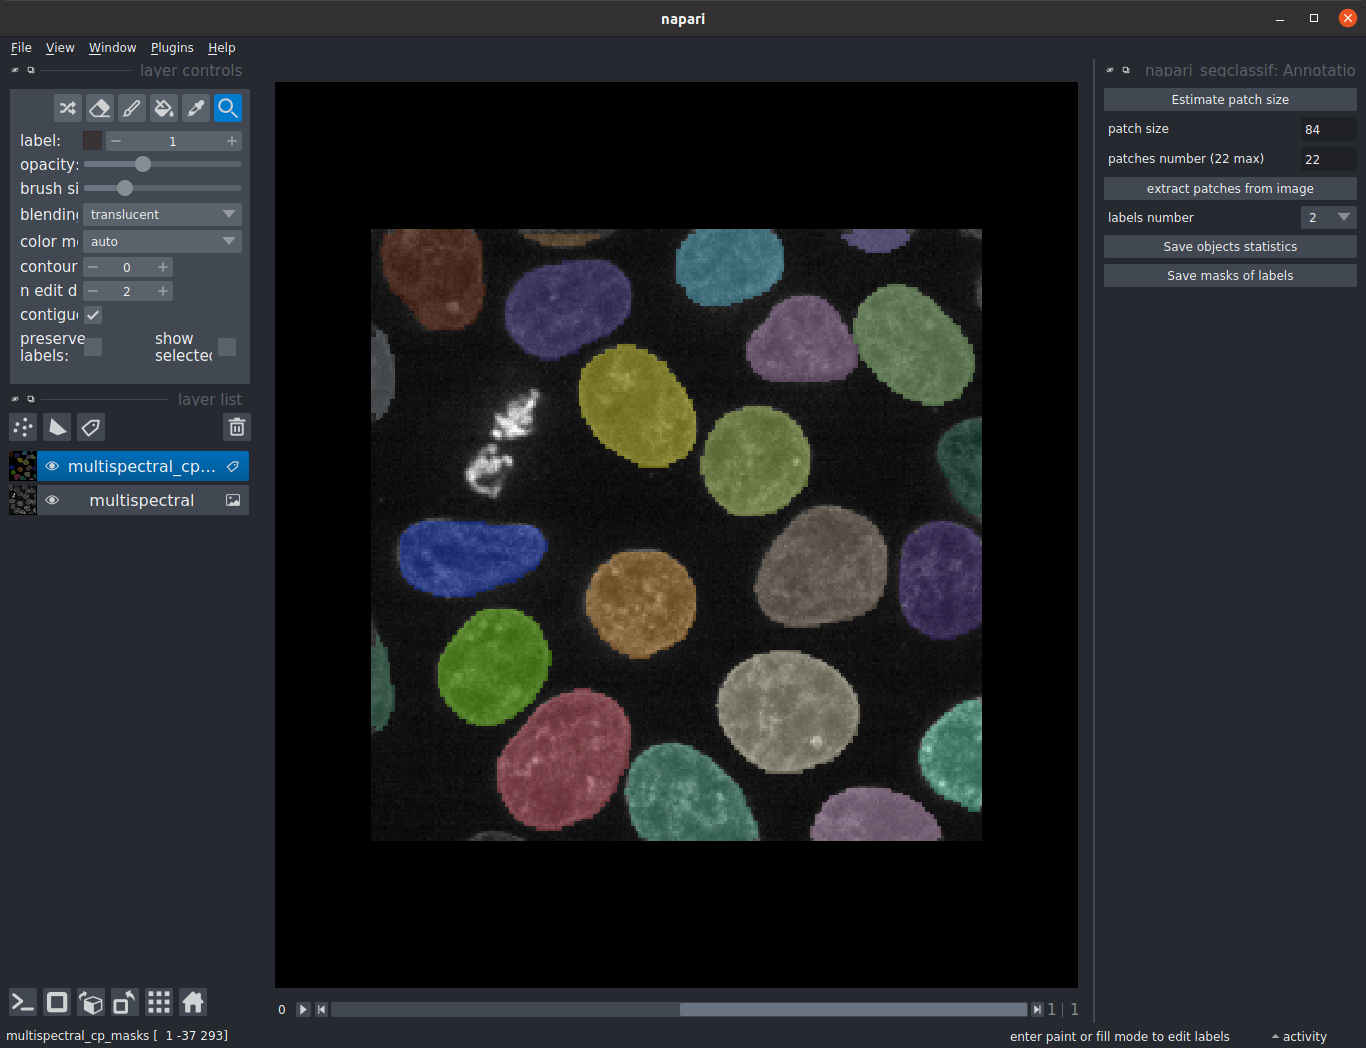
\includegraphics[scale=0.2]{Figures/annotations.png}
  \caption{Annotation interface}
  \label{labelization}

\end{figure}


\begin{figure}[htp!]
 \centering
 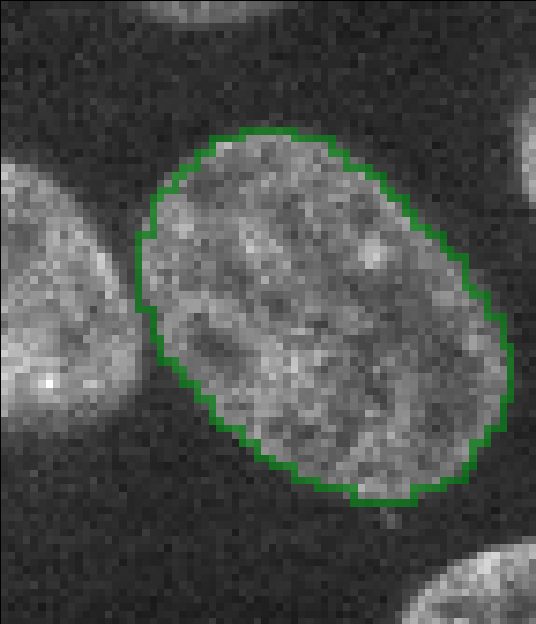
\includegraphics[scale=0.2]{Figures/patch.png}
  \caption{Visualisation of a patch to be annotated}
  \label{patch}

\end{figure}

Apporter un outil permettant de "trier" les résultats de segmentation, de façon manuelle ou automatique. 
Cet outil permet de faire plusieurs choses:
\begin{itemize}
  \item Annotation: This first sub-plugin can be seen as a simple facilitation tool for manual annotation of objects into different classes. It can also be used as a tool to annotate a minimal database that will be used to train a classification model. 
  \item Entraînement de réseaux de classification. 
  \item Utilisation des réseaux entraînés pour la prédiction lorsqu'il y a de larges collections.
\end{itemize}


\subsection{The choice of Napari}

Napari VS Fiji.
outils open-source, intuitifs et user-friendly sous la forme de plugins pour des logiciels libres tels que Fiji \cite{schindelin2012fiji} ou plus récemment 


\subsection{The annotation mode}

\subsection{The training mode}

Parler de Deep Image Prior (i.e. on peut entraîner avec peu de labels, rasoir d'Ockham, Yann Ollivier).

\subsection{The prediction mode}


\section{Numerical Experiments}
\label{sec:experiments}




\section{Conclusion}
\label{sec:conclusion}




% To start a new column (but not a new page) and help balance the last-page
% column length use \vfill\pagebreak.
% -------------------------------------------------------------------------
\vfill
\pagebreak

% \section{REFERENCES}
% \label{sec:ref}

% References should be produced using the bibtex program from suitable
% BiBTeX files (here: refs). The IEEEbib.bst bibliography
% style file from IEEE produces unsorted bibliography list.
% -------------------------------------------------------------------------
\bibliographystyle{IEEEbib}
\bibliography{refs}

\end{document}
























%%%%%%%%%%%%%%%%%%%%%%%%%%%%%%%%%%%%%%%%%%%%%%%%%%%%%%%%%%%%%%%%%%%%

La dernière décennie a rendu la segmentation automatique d'images bio-médicales bien plus accessible à des utilisateurs non experts en traitement du signal. 
Ceci est largement dû aux progrès en apprentissage automatique et notamment en apprentissage par réseaux de neurones convolutionnels. Ils permettent notamment d'éviter le réglage de nombreux hyperparamètres dont le tuning est difficile et dont la signification est obscure pour les non initiés. 
A titre d'exemple, on peut citer des outils récents, puissants et populaires tels que Ilastik \cite{berg2019ilastik}, Cellpose \cite{stringer2021cellpose}, StarDist \cite{fazeli2020automated} ou plus récemment Deep-ImageJ \cite{gomez2021deepimagej}. 

Malheureusement, les résultats de segmentation -- aussi bons soient-t'ils -- sont rarement exploitables directement pour répondre à des questions biologiques. Il est en effet fréquent qu'il faille  classifier les objets détectés pour effectuer des analyses statistiques apportant un sens concret aux résultats. En un sens, ces outils ont résolu une partie du problème, mais une partie importante et difficile de l'analyse reste inaccessible.

L'objectif de ce travail est de continuer à combler le fossé entre les progrès méthodologiques et les end-users, en fournissant des outils faciles d'utilisation pour la classification des résultats de segmentation.
Ces outils prennent la forme d'un plugin Napari \cite{perkel2021python}, qui est un nouvel outil de visualisation d'images complexes sous Python.

